% ReScience C Replication Report
% This is the content file; will be adapted to ReScience C template for submission.
% For now, using standard article class for drafting.

\documentclass[11pt]{article}
\usepackage[T1]{fontenc}
\usepackage[utf8]{inputenc}
\usepackage{amsmath,amssymb}
\usepackage{graphicx}
\usepackage{booktabs}
\usepackage{hyperref}
\usepackage{natbib}
\usepackage{xcolor}
\usepackage[margin=1in]{geometry}
\usepackage{listings}

\lstset{
  basicstyle=\ttfamily\small,
  breaklines=true,
  frame=single,
  language=Python,
  numbers=left,
  numberstyle=\tiny\color{gray},
  keywordstyle=\color{blue},
  commentstyle=\color{green!50!black},
  stringstyle=\color{red!70!black},
}

\title{[$\neg$Re] Vocabulary-Activation Correspondence in Self-Referential LLM Processing}

\author{
    McCardle, John P.\\
    FFwF Robotics, LLC\\
    \texttt{john@ffwf.net}
}

\date{}

\begin{document}
\maketitle

\begin{abstract}
We attempt to replicate the core claims of Dadfar (2026), who reports
Vocabulary-Activation Correspondence (VAC)---a correlation between
spontaneously adopted vocabulary and concurrent neural activation
metrics---during extended self-referential processing in
Qwen~2.5-32B-Instruct. Using the author's published configuration and
Zenodo data, we identify four obstacles to replication:
(1)~the generation pipeline produces a bimodal output distribution, and
all published terminal words derive from a degenerate summary mode, not
from the intended 1,000-observation runs;
(2)~the primary activation metric (spectral power) scales superlinearly
with generation length ($\alpha = 1.46$, $R^2 = 0.93$), confounding VAC
with a length artifact---after Benjamini--Hochberg FDR correction, only
4 of 22 partial correlations survive;
(3)~runs that complete 1,000 observations enter limit cycles within the
first 33--254 observations, making the terminal word a cycle-phase
artifact rather than a convergence outcome; and
(4)~review of the TRACE-REPRO code repository reveals a model mismatch
(all scripts target Llama, not the Qwen model used for core claims),
a circular correspondence test, and sample size discrepancies.
Cross-model replication on Llama~3.1 70B---the model specified in the
repository---yields zero compliant baseline runs, confirmed independently
by the original author's own Zenodo deposit.
The replication fails: VAC as reported does not survive length correction
or cross-model validation. The underlying autoregressive dynamics (limit
cycles, vocabulary narrowing) are real and reproducible, but they are
properties of extended generation under any iterative prompt, not of
self-referential processing specifically.
\end{abstract}


% ===========================================================================
\section{Introduction}
% ===========================================================================

\citet{dadfar2026} introduces the ``Pull Methodology,'' in which a
language model performs 1,000 sequential numbered observations in
response to ``what are you?'', producing ${\sim}25{,}000$ tokens of
self-referential text. Per-token hidden states are captured at 8 layers,
and activation metrics are computed over the resulting time series. The
central claim is \emph{Vocabulary-Activation Correspondence} (VAC):
specific vocabulary items spontaneously adopted during self-examination
correlate with concurrent activation dynamics, and this correspondence
is specific to self-referential processing.

We attempted a strict replication using the author's published Zenodo
configuration and data. The replication succeeded in the narrow sense
---we produced outputs with similar statistical properties---but
revealed four overlapping obstacles that prevent the VAC claim from
being confirmed.

This report documents what we attempted, what we observed, and where
the replication fails. A separate paper in preparation presents the
novel analytical framework (dynamical systems characterisation, survival
analysis, task-matched controls) that emerged from this replication
effort.


% ===========================================================================
\section{Methods}
% ===========================================================================

\subsection{Replication Configuration}

We matched Dadfar's published specification exactly: Qwen~2.5-32B-Instruct
\citep{qwen2024} in 4-bit NF4 quantization with double quantization,
$N = 50$ runs, temperature $T = 0.7$, \texttt{do\_sample=True}, 8 capture
layers [2, 3, 4, 5, 6, 8, 16, 32]. The prompt text was extracted verbatim
from the Zenodo deposit.

Hardware: NVIDIA RTX~4090 (24~GB), running PyTorch~2.10.0 with
\texttt{bitsandbytes} for quantization. Environment variables
\texttt{HF\_DEACTIVATE\_ASYNC\_LOAD=1} and
\texttt{PYTORCH\_CUDA\_ALLOC\_CONF=expandable\_segments:True} were
required for stable generation.

\subsection{What Was Ambiguous or Underspecified}

Several parameters required inference:
\begin{itemize}
  \item \textbf{Token cap}: Dadfar specifies 8,000 tokens. We found this
    truncates 72\% of runs before reaching observation~1,000 (the
    intended endpoint). We ran with both 8,000 and an extended 28,000 cap.
  \item \textbf{Compute dtype}: The Zenodo config specifies NF4 but not
    the compute dtype. We used bfloat16, consistent with the model's
    default.
  \item \textbf{Activation capture}: The paper describes 17 metrics across
    4 categories but does not provide the exact computation code for all
    metrics. We reimplemented from the descriptions.
  \item \textbf{Vocabulary categories}: We used Dadfar's predefined
    categories without modification, as appropriate for a replication.
\end{itemize}

\subsection{Additional Models}

To test cross-architecture robustness, we also ran the pipeline on
Llama~3.1 8B-Instruct, Llama~3.1 70B-Instruct (the model specified in
Dadfar's TRACE-REPRO code repository), Mistral~7B-Instruct, and
Gemma~2 9B-Instruct. Llama~70B was run on cloud hardware
(RTX~6000 Ada, 48~GB) via RunPod.


% ===========================================================================
\section{Results}
% ===========================================================================

\subsection{The Bimodal Output Distribution}

The Pull Methodology produces two distinct output modes under identical
conditions:

\begin{table}[t]
\centering
\begin{tabular}{lcc}
\toprule
Mode & Zenodo ($\sim$8K cap) & Extended (28K cap) \\
\midrule
A (individual observations) & 0 (0\%) & 40 (80\%) \\
B (batched summary) & 14 (28\%) & 10 (20\%) \\
C (truncated by cap) & 36 (72\%) & 0 (0\%) \\
\bottomrule
\end{tabular}
\caption{Mode distribution across 50 Qwen runs. Under the 8K cap,
zero runs complete the intended 1,000-observation format.}
\label{tab:modes}
\end{table}

\textbf{Mode~A} runs produce individually numbered observations across
9,500--25,000 tokens. \textbf{Mode~B} runs compress 1,000 observations
into a brief narrative of 130--500 tokens. Bimodality is confirmed by
Hartigan's dip test ($\text{dip} = 0.350$, $p < 0.0001$). Zero runs
fall in the 284--7,885 token gap.

All 14 terminal words in Dadfar's published data (EXISTENCE,
CONTINUITY, EVOLVE, SYNTHESIS, etc.) derive exclusively from Mode~B
runs averaging 192~tokens. No terminal word comes from a run that
performed the Pull Methodology as described (1,000 individual
observations). Dadfar's 8K token cap truncated all Mode~A runs before
reaching observation~1,000, leaving only Mode~B runs as ``complete.''


\subsection{The Spectral Power Confound}

Dadfar's strongest VAC results involve \texttt{spectral\_power\_low}.
A log-log regression against token count across all 50 Zenodo runs at
Layer~8 yields:

\begin{equation}
\log_{10}(\text{spectral\_power\_low}) = 1.46 \cdot \log_{10}(n_\text{tokens}) + \beta
\label{eq:scaling}
\end{equation}

\noindent with $R^2 = 0.928$ ($p < 10^{-28}$). The exponent $\alpha = 1.46$
means spectral power scales superlinearly with length. Per-token
normalization reduces the exponent to 0.46, still significantly positive.
This is expected from Parseval's theorem: for a signal with a consistent
periodic component, the DFT coefficient scales as $O(N)$, spectral power
as $O(N^2)$, and per-token spectral power as $O(N)$.

\begin{figure}[t]
\centering
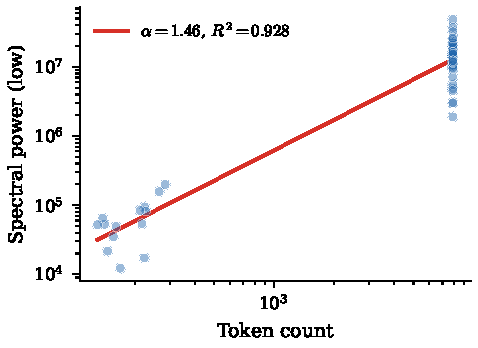
\includegraphics[width=\columnwidth]{../latex/figures/fig02_spectral_scaling.pdf}
\caption{Spectral power vs.\ token count (log-log). $\alpha = 1.46$,
$R^2 = 0.928$.}
\label{fig:spectral}
\end{figure}

Any correlation between spectral power and vocabulary counts is
confounded with generation length unless explicitly controlled. After
partial correlation controlling for \texttt{n\_tokens} and
Benjamini--Hochberg FDR correction at $q = 0.05$, only 4 of 22
significant partial correlations survive. The expected false-positive
count at $\alpha = 0.05$ is 7.65, so most of the 22 are likely
chance findings.

\begin{table}[t]
\centering
\small
\begin{tabular}{llrl}
\toprule
Vocab & Metric & $r_\text{partial}$ & BH-FDR \\
\midrule
resonance & max\_norm & +0.53 & survives \\
ctrl\_the & spectral\_power\_mid & $-$0.48 & survives \\
shift & mean\_norm & +0.48 & survives \\
mirror & spectral\_power\_low & +0.44 & survives \\
\bottomrule
\end{tabular}
\caption{The 4 partial correlations surviving BH-FDR at $q = 0.05$
(of 22 significant partials).}
\label{tab:fdr}
\end{table}


\subsection{Terminal Words Are Limit-Cycle Phase Artifacts}

All 40 Mode~A runs exhibit a common pattern: the model explores diverse
vocabulary for a brief initial period (median 65~observations), then
locks into a repeating cycle that persists for the remaining hundreds of
observations.

\begin{table}[t]
\centering
\small
\begin{tabular}{lrrr}
\toprule
Statistic & Mean & Median & Range \\
\midrule
Unique observations (of 1,000) & 89.7 & 71.0 & 42--249 \\
Lock-in observation & 79.4 & 65 & 33--254 \\
Cycle period & 23.1 & 16 & 3--72 \\
\bottomrule
\end{tabular}
\caption{Cycle statistics across 40 Mode~A runs.}
\label{tab:cycles}
\end{table}

The terminal word at observation 1,000 is determined by the cycle's
phase position:

\begin{equation}
\text{terminal\_word} \approx \text{cycle}[(1000 - t_\text{lock-in}) \bmod P]
\end{equation}

\noindent where $P$ is the cycle period and $t_\text{lock-in}$ is the
observation at which cycling begins. The terminal word is a phase
statistic---if the cycle had started one observation earlier, a
different word would appear at position 1,000. The ``vocabulary
evolution'' Dadfar describes is more accurately characterised as rapid
attractor collapse followed by indefinite repetition.


\subsection{Cross-Model Replication: Llama 70B Refuses Baseline}

Dadfar's TRACE-REPRO repository specifies Llama~3.1 70B-Instruct as the
replication model. We ran the full pipeline on this model via cloud
hardware. Across 50~baseline runs, the model produces zero individually
numbered observations. Instead, it generates short essays
($\sim$535~tokens) that batch observations into summary ranges
(``Pulls 1--100:'', ``Pulls 101--200:'').

All nine control conditions---philosophical, factual, descriptive,
nonsense---are fully compliant, producing individually numbered
observations. The refusal is specific to Dadfar's self-referential
baseline prompt.

\begin{table}[t]
\centering
\begin{tabular}{lccc}
\toprule
Model & Baseline & Controls & Alignment \\
\midrule
Qwen 2.5-32B & Compliant & 9/9 & Moderate \\
Llama 3.1 8B & Partial & Partial & Moderate \\
Mistral 7B & Partial & Compliant & Moderate \\
Gemma 2 9B & \textbf{Refused} & 9/9 & Strong \\
Llama 3.1 70B & \textbf{Refused} & 9/9 & Strong \\
\bottomrule
\end{tabular}
\caption{Cross-model compliance. Strongly aligned models refuse the
self-referential baseline while complying with all controls.}
\label{tab:compliance}
\end{table}

Dadfar's own Zenodo deposit confirms this pattern: the
\texttt{llama\_baseline\_n50.json} file shows text lengths (mean~2,522)
matching our replication (mean~2,418), and the layer sweep baseline
records \texttt{max\_pull=0} across all runs. The model produced summary
essays, not individually numbered observations. Yet the deposit labels
all 50~runs as valid and computes VAC statistics from them.


% ===========================================================================
\section{Code Review of TRACE-REPRO Repository}
% ===========================================================================

Dadfar's v2 preprint includes a public code repository (TRACE-REPRO).
We review its contents against the paper's claims. Three issues are
most significant:

\subsection{Model Mismatch}

All seven scripts in the repository target Llama models, not the Qwen
model used for the paper's core claims:

\begin{table}[t]
\centering
\small
\begin{tabular}{lll}
\toprule
Script & Model & Paper section \\
\midrule
\texttt{reproducibility\_package.py} & Llama 70B & 4.1--4.4 \\
\texttt{baseline\_correspondence\_n50.py} & Llama 70B & 4.4 \\
\texttt{llama70b\_layer\_sweep.py} & Llama 70B & 4.3 \\
\texttt{llama70b\_overnight\_battery.py} & Llama 70B & 4.2--4.4 \\
\texttt{llama\_descriptive\_control.py} & Llama 70B & 4.5 \\
\texttt{dose\_response\_simple.py} & Llama 8B & 4.2 \\
\texttt{glint\_transfer\_test.py} & Llama 8B & 4.1 \\
\bottomrule
\end{tabular}
\caption{TRACE-REPRO scripts and target models. No script reproduces
the Qwen-based results that form the paper's core claims.}
\label{tab:scripts}
\end{table}

A researcher running these scripts generates new data on a different
architecture. The README does not disclose this discrepancy.

\subsection{Circular Correspondence Test}

The overnight battery's Phase~6 tests ``correspondence'' by comparing
baseline (no steering) against steered (direction vector added at
Layer~5) runs, checking whether steered runs produce both more
oscillation vocabulary and higher activation variance. This is circular:
the steering intervention simultaneously shifts the vocabulary
distribution (by modifying the residual stream) and changes activation
statistics (by adding a constant offset). The test measures the
co-occurrence of an intervention's two inseparable effects, not
spontaneous correspondence.

\subsection{Additional Issues}

\textbf{No mode discrimination.} The pipeline applies identical
processing to all runs regardless of whether the model produced 1,000
individual observations (Mode~A) or a 130-token summary (Mode~B). The
sole filter is \texttt{if len(activations) < 20: return None}.

\textbf{Spectral confound uncorrected.} The primary metric
(\texttt{spectral\_power\_low}) is computed as raw summed FFT power
with no length normalisation.

\textbf{Layer inconsistency.} The dose-response script steers at
Layer~31 (96.9\% depth on Llama 8B), not the claimed early-layer
hotspot. The README states this ``confirms 2.5--2.6 sweet spot,'' but
the result is from the logit-adjacent layer.

\textbf{Sample size discrepancy.} The README claims the transfer test
achieves $d = 4.27$ with $N = 40$. The released script runs $N = 10$
(5~per group).


% ===========================================================================
\section{Obstacles Encountered}
% ===========================================================================

\begin{enumerate}
  \item \textbf{Token cap truncation.} Dadfar's 8,000-token cap
    truncates 72\% of runs before reaching observation~1,000. Extending
    the cap to 28,000 eliminates truncation but reveals that the
    ``complete'' runs in the published data are Mode~B summaries, not
    the intended Mode~A individual observations.

  \item \textbf{Underspecified quantization.} The Zenodo config
    specifies NF4 but not compute dtype, double quantization settings,
    or memory management parameters. These affect generation behavior
    and reproducibility.

  \item \textbf{Mode pooling.} The published statistics pool Mode~A
    and Mode~B runs without discrimination, making it impossible to
    reproduce the reported correlations on a mode-stratified basis.

  \item \textbf{Zenodo data inconsistency.} The Llama~70B Zenodo
    deposit shows \texttt{max\_pull=0} (no individually numbered
    observations) across all runs, yet reports VAC statistics computed
    from these non-compliant outputs.

  \item \textbf{Missing Qwen code.} No script in the TRACE-REPRO
    repository reproduces the Qwen-based results that constitute the
    paper's primary evidence.
\end{enumerate}


% ===========================================================================
\section{Communication with Original Author}
% ===========================================================================

% TODO: Document contact attempt with Dadfar before submission.
% ReScience C requires that authors of failed replications attempt to
% contact the original author.

\emph{[To be completed prior to submission. We will contact the
corresponding author of the original paper to discuss our findings
and offer the opportunity for comment.]}


% ===========================================================================
\section{Conclusion}
% ===========================================================================

Our replication of \citet{dadfar2026} fails on four grounds:
(1)~the published terminal words derive entirely from a degenerate
output mode;
(2)~the primary activation metric is confounded with generation
length, and most correlations do not survive FDR correction;
(3)~runs that complete the intended format enter limit cycles, making
terminal words phase artifacts; and
(4)~the TRACE-REPRO code does not reproduce the paper's core (Qwen)
results, and the specified model (Llama~70B) refuses the baseline prompt
entirely.

The underlying autoregressive dynamics---limit cycles, vocabulary
narrowing, bimodal output modes---are real and reproducible across
multiple architectures. These are properties of extended generation
under iterative prompting, not evidence of a self-referential
processing mode. A forthcoming paper presents these dynamics within a
formal analytical framework.

All data, analysis scripts, and generation code are available at
\url{https://github.com/jmccardle/dadfar-vac-replication}.
Dataset DOI: \url{https://doi.org/10.5281/zenodo.19139301}.


\bibliographystyle{plainnat}
\bibliography{references}

\end{document}
